\documentclass[12pt]{article}
\usepackage{amsmath}
\usepackage{amssymb}
\usepackage{amsthm}
\usepackage{amsfonts}
\usepackage{graphicx}
\usepackage{textcomp}
\usepackage{hyperref}
\usepackage{tikz}
\usepackage{enumitem}
\usepackage{mathtools}
\usepackage{float}
\usepackage{cleveref}
\usepackage{hyperref}
\usepackage{csquotes}

\begin{document}

\title{MACM 101 Chapter 1.1}
\author{Alexander Ng}
\date{Friday, September 13, 2024}

\maketitle

% \section{Chapter Summary}

% \begin{itemize}
%   \item Propositional Logic
%     \subitem The Language of Propositions
%     \subitem Applications
%     \subitem Logical Equivalences and Implication
%     \subitem The Laws of Propositional Logic
%
%   \item Predicate Logic
%     \subitem The Language of Quantifiers
%     \subitem Nested Quantifiers
%
%   \item Proofs
%     \subitem Rules of Inference
%     \subitem Proof Methods
%     \subitem Proof Strategy
% \end{itemize}

This document covers Rosen 1.0 and 1.1.

\pagebreak
\section{Definitions}

\subsection{Deduction/Deductive Logic}

Deduction is the process of deriving a conclusion from a given set of axioms 
or premises. In Logic, we start from the ground (axioms) and work our way up to
the conclusion.

\subsection{Truth Value}

A truth value can be either true or false, but not both. This comes from the
\textit{principium tertii eclusi} of Aristotle.

\subsubsection{True and False}

We will use 1 and 0 to denote true and false, respectively.

\subsubsection{Unknown Truth Value}

The proposition $u$ is \textit{unknown truth value}.

\subsection{Proposition}

A proposition is a declarative sentence (or statement) that possesses truth value.

\subsubsection{Notation}

Lowercase letters denote primitive propositions, and uppercase letters denote
complex propositions.

Primitive propositions are:

\begin{itemize}
\item Propositions that cannot be decomposed into anything simpler
\item $p: 3 + 5 = 8$
\item $q: \text{It is raining}$
\end{itemize}

\subsection{Examples of things that are not propositions}

\begin{itemize}
\item $p:$ Sit down! $\to$ not a proposition because it is not a declarative
\item $q:$ The statement you are reading is now false. $\to$ not a proposition
  because it is a contradiction.
\item $r:$ The number $x$ is an integer. $\to$ not a proposition because it 
  contains an unspecified variable, which means it's truth value cannot be
  definitively determined without additional information.
\end{itemize}

\subsection{Syntactics and Semantics}

Syntatic reasoning is what can be shown. 

Syntax ~= grammar (rules of sentance construction), the structure of propositions

Semantics reasoning is what is true

Semantics ~= meaning (truth value), the truth value/tables of propositions

\subsection{Literals}

A \textit{literal} is either a primitive proposition or its negation (some
textbooks use ~ to denote a literal)

\section{Operator Syntax}

\begin{enumerate}
  \item Negation - $\neg$ \\
    $q:$ it is raining, $\neg q:$ it is not raining\\
  Everything in this list other than $\neg $  is known as a \textit{logical connective}
  \item Conjunction - $\land$ - Logical and\\
    $p \land q:$ it is raining and it is sunny \\
    $p \land \neg q:$ it is raining and it is not sunny
  \item Disjunction - $\lor$ - Inclusive Or\\
    $p \lor q:$ it is raining or it is sunny \\
    $p \lor \neg q:$ it is raining or it is not sunny
  \item Disjunction - $\oplus$ - Exclusive Or\\
    $p \oplus q:$ it is raining xor it is sunny \\
    $p \oplus \neg q:$ it is raining xor it is not sunny\\
    XOR is generally what is meant in english sentences like "the meal comes
    with either soup or salad"
  \item Implication - $\to$ - "If, then"
  \item Biconditional - $\leftrightarrow$ - "If and only if"
\end{enumerate}

Nobody knows why OR and XOR are both called Disjunction

All propositions formed with logical connectives are called \textit{compound propositions},
as opposed to \textit{primitive propositions}

Compound propositions need not have causal
relations between atomic components (they
can sound nonsensical and still be valid) –
material implication as opposed to causal
implication, which lacks temporal ordering. (straight from the slides, p. 34)

\section{Logical Equivalences}

\begin{figure}[H]
    \centering
    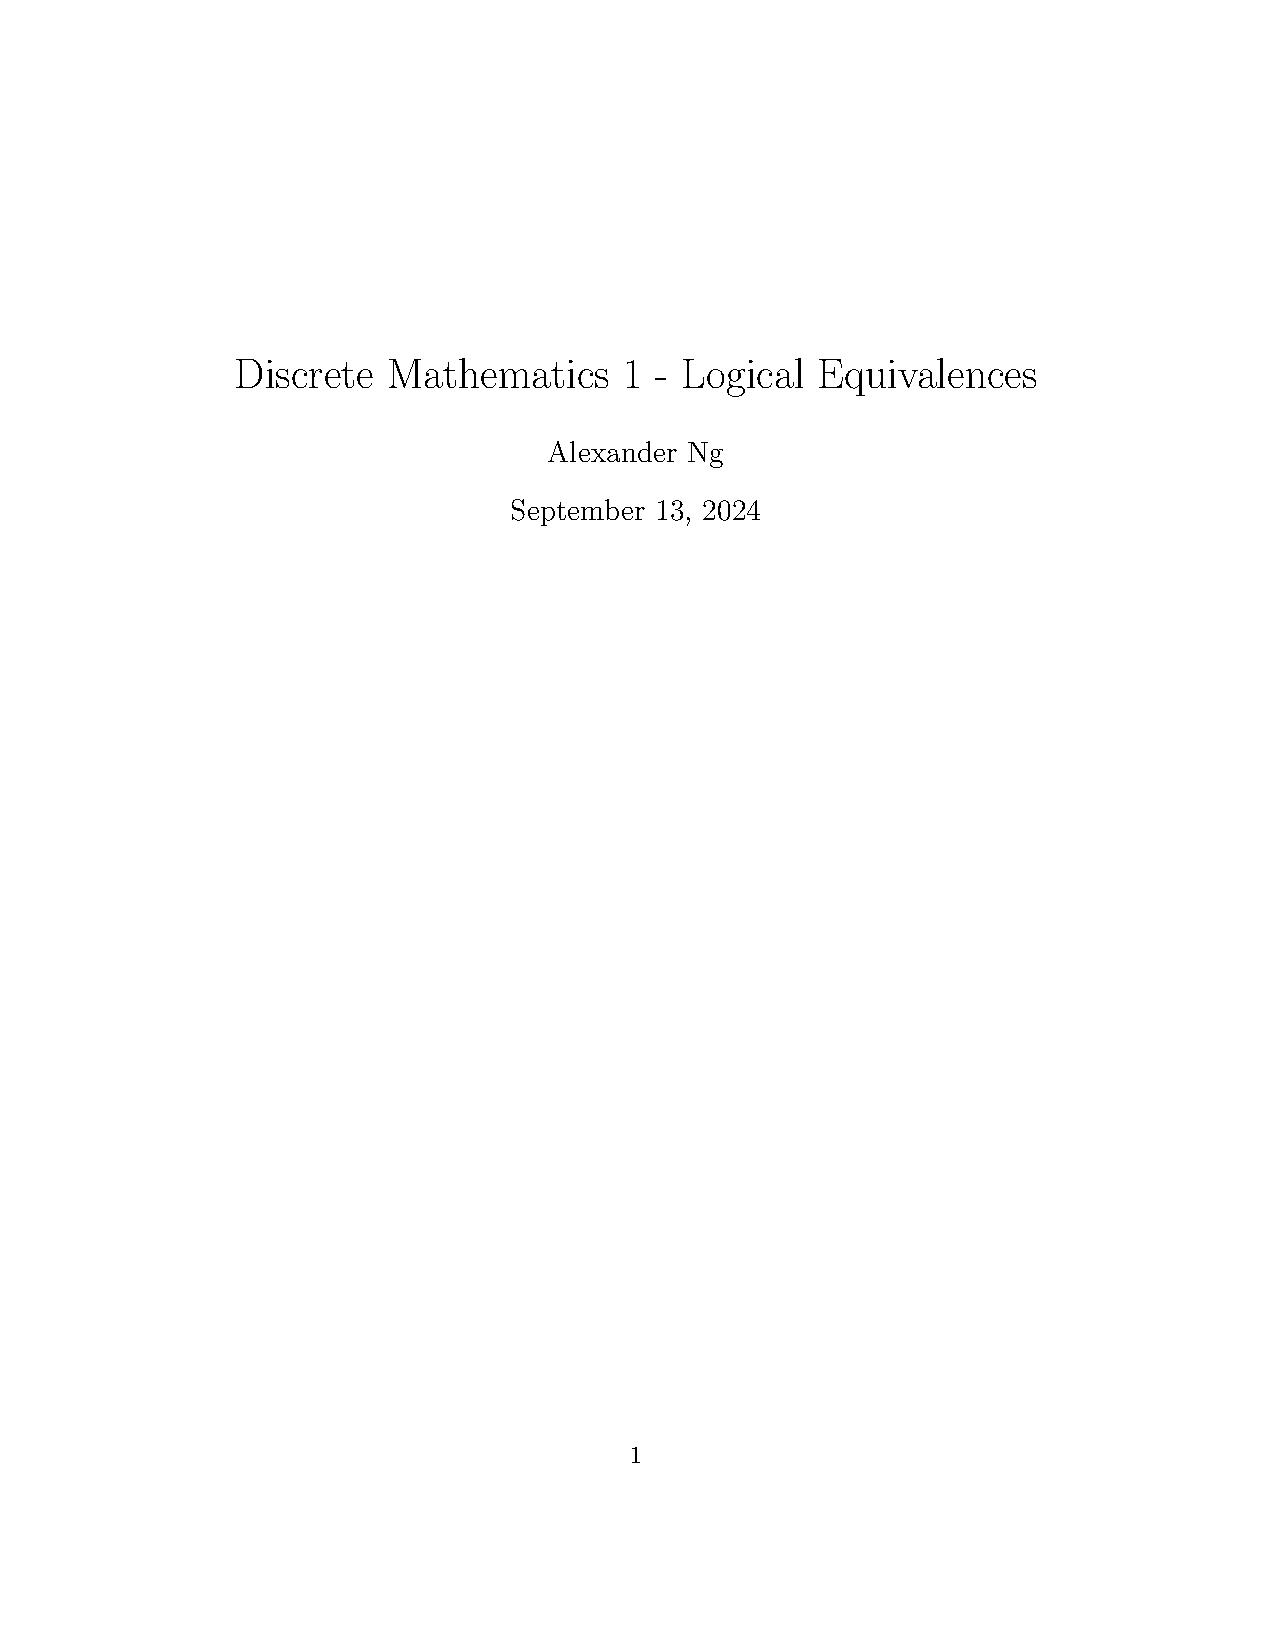
\includegraphics[width=0.8\textwidth]{"./Logical Equivalences.jpg"}
    \caption{Logical Equivalences}
    \label{fig:logical_equivalences}
\end{figure}

\begin{figure}[H]
    \centering
    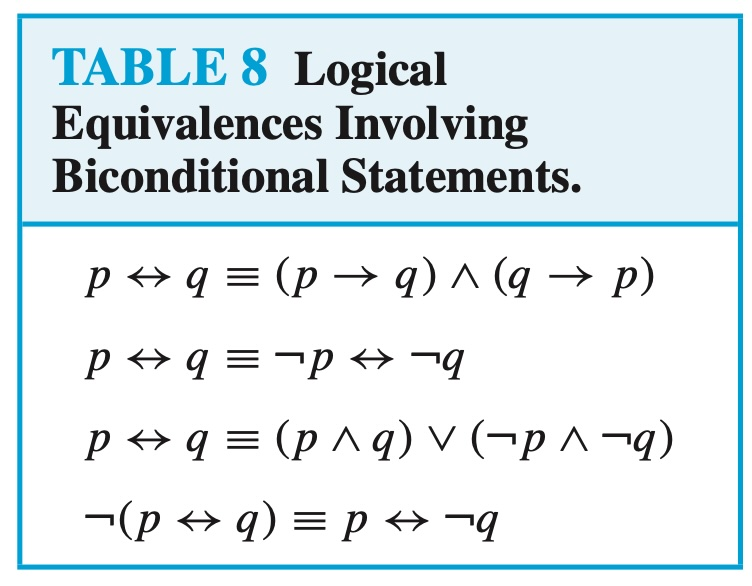
\includegraphics[width=0.4\textwidth]{"./Logical Equivalences Involving Biconditional Statements.jpg"}
    \caption{Logical Equivalences Involving Biconditional Statements}
    \label{fig:logical_equivalences_biconditional}
\end{figure}

\begin{figure}[H]
    \centering
    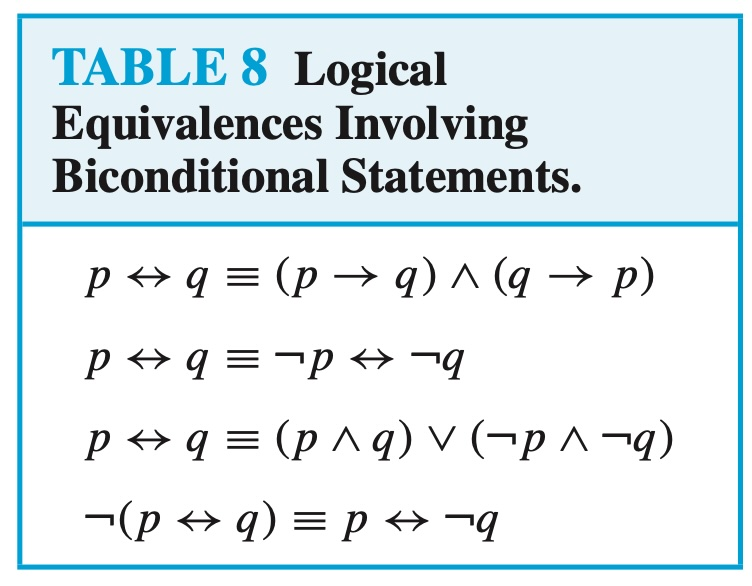
\includegraphics[width=0.4\textwidth]{"./Logical Equivalences Involving Biconditional Statements.jpg"}
    \caption{Logical Equivalences Involving Conditional Statements}
    \label{fig:logical_equivalences_conditional}
\end{figure}

\section{Semantics}

Basically, all semantics is is truth tables.

\subsection{Negation, $\neg$}

\[
\begin{array}{|c|c|}
\hline
p & \neg p \\
\hline
T & F \\
F & T \\
\hline
\end{array}
\]

\subsection{Logical Connectives}

\begin{enumerate}
  \item Conjunction - $\land$ - Logical AND
  \item Disjunction - $\lor$ - Logical OR
  \item Exclusive Or - $\oplus$ - Exclusive OR
  \item Implication - $\to$ - Material Implication
  \item Biconditional - $\leftrightarrow$ - Biconditional
\end{enumerate}

\[
\begin{array}{|c|c|c|c|c|c|c|}
\hline
p & q & p \land q & p \lor q & p \oplus q & p \to q & p \leftrightarrow q \\
\hline
1 & 1 & 1 & 1 & 0 & 1 & 1 \\
1 & 0 & 0 & 1 & 1 & 0 & 0 \\
0 & 1 & 0 & 1 & 1 & 1 & 0 \\
0 & 0 & 0 & 0 & 0 & 1 & 1 \\
\hline
\end{array}
\]

\subsection{Extra Context for Material Implication}

A wide range of terminology exists to describe material implication.

\begin{figure}[H]
    \centering
    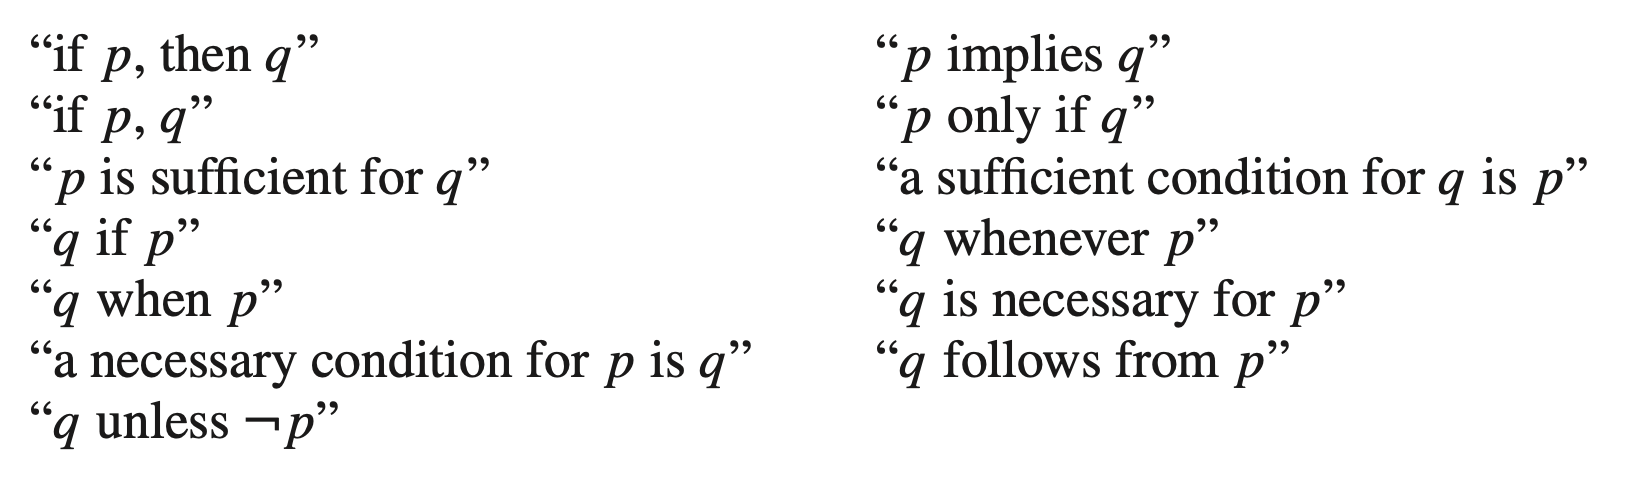
\includegraphics[width=0.8\textwidth]{"./p_implies_q.png"}
    \caption{Ways to Express $p \to q$}
    \label{fig:p_implies_q}
\end{figure}

Note that Material Implication does not depend on any relationship between the
meanings of the two propisitions involved, but only the \textit{truth values} of
the propositions.

\subsubsection{Necessary Conditions (implication)}

For a normal car to run, it is necessary that there is fuel in the tank,
its spark plugs are properly adjusted, its oil pump is working, etc.

If the car runs, then every one of the conditions must be fulfilled.

All of these propositions are $p \to q$

Let $p$ be the statement "the car runs"

Let $q$ be the other statement

\begin{enumerate}
\item If the car runs, then fuel must be in the tank. $(p \to q)$
\item If the car runs, its spark plugs must be properly adjusted. $(p \to q)$
\item If the car runs, its oil pump must be working. $(p \to q)$
\end{enumerate}

From this, you can see why material implication is defined by 
$\neg (p \land \neg q) \equiv \neg p \lor q$. I think that $\neg (p \land \neg q)$
makes a lot more sense than $\neg p \lor q$ when you read it out loud. With
this definition, you can clearly visualize the truth table. Try thinking about
(not (p land not q)) and look at the truth table.

% 1.1 PDF p.48 (still c1.1 in the book)

\subsubsection{Sufficient Conditions (implication)}

For a purse to contain over a dollar, it would be sufficient for it to contain
101 pennies, 21 nickels, 11 dimes, 5 quarters, etc.

If any one of these circumstances is obtained, the specified situation will
be realized.

\subsubsection{Hints (wording)}

\begin{enumerate}
  \item "p is a \textbf{sufficient condition} for q"\\
    $p \to q$ (q is a necessary condition for p)
  \item "p is a \textbf{necessary condition} for q"\\
    $q \to p$ (q is a sufficient condition for p)
  \item Given any sentence saying something is \textit{necessary} or 
    \textit{sufficient}, it is always:\\
    sufficient $\to$ necessary
\end{enumerate}

$p\to q$ can read as any one of the phrases highlighted in
\hyperref[fig:p_implies_q]{Figure~\ref*{fig:p_implies_q}}

\subsubsection{The Four Types of Implication}

There are 4 types of implication

\begin{enumerate}
\item \textbf{Logical Implication} - the consequent follows logically from its
  antecedent (a.k.a. material implication)
  \subitem If all humans are mortal and Socrates is a human, then Socrates is
    mortal.
\item \textbf{Definitional Implication} - the consequent follows the antecedent
  by definition.
  \subitem If Leslie is a Bachelor, then Leslie is unmarried.
\item \textbf{Causal Implication} The connection between antecedent and 
  consequent is discovered empirically (temporal ordering is implicit)
  \subitem If I put X in acid, then X will turn red.
\item \textbf{Decisional Implication} - A decision of the speaker to behave in
  the specified way under the specified circumstances.
  \subitem If we lose the game, then I'll eat my hat.
\end{enumerate}

For Propositional Logic, we will only be concerned with logical implication
(material implication).

\subsection{Order of Operations for Propositions}

\[
\begin{array}{|c|c|}
\hline
Operator & Precedence \\
\hline
\neg & 1 \\
\land & 2 \\
\lor & 3 \\
\to & 4 \\
\leftrightarrow & 5 \\
\hline
\end{array}
\]

% please include \oplus at some point in this table

\section{Bit Strings}

A \textbf{bit string} is a sequence of zero or more bits. 

We can extend our bit operations to bit strings. We define the 
\textbf{bitwise OR}, \textbf{bitwise AND}, and \textbf{bitwise XOR} of two bit
strings of the same length to be the strings that have, as their bits, the
\textbf{OR}, \textbf{AND}, and \textbf{XOR} of the corresponding bits in the
two strings, respectively. (Pearce, 60)

Translated into plain English, the bitwise extension of the logical operations
means to take each corresponding bit in the two strings and apply the logical
operation to them.

Bitwise literally means \enquote{by bit}, so the bitwise extension of the
logical operations in this way are called \textbf{bitwise logical operations}.

If you need examples of this, please refer to Pearce, 60 or Rosen, 12.

\end{document}
